\documentclass[twocolumn,a4j]{jsarticle}
\setlength{\topmargin}{-20.4cm}
\setlength{\oddsidemargin}{-10.4mm}
\setlength{\evensidemargin}{-10.4mm}
\setlength{\textwidth}{18cm}
\setlength{\textheight}{26cm}

\usepackage[top=15truemm,bottom=20truemm,left=20truemm,right=20truemm]{geometry}
\usepackage[latin1]{inputenc}
\usepackage{amsmath}
\usepackage{amsfonts}
\usepackage{amssymb}
\usepackage[dvipdfmx]{graphicx}
\usepackage[hang,small,bf]{caption}
\usepackage[subrefformat=parens]{subcaption}
\usepackage[dvipdfmx]{color}
\usepackage{listings}
\usepackage{listings,jvlisting}
\usepackage{geometry}
\usepackage{framed}
\usepackage{color}
\usepackage[dvipdfmx]{hyperref}
\usepackage{ascmac}
\usepackage{enumerate}
\usepackage{tabularx}
\usepackage{cancel}
\usepackage{scalefnt}
\usepackage{overcite}
\usepackage{otf}
\usepackage{multicol}
\usepackage[geometry]{ifsym}

\renewcommand{\figurename}{Fig.}
\renewcommand{\tablename}{Table }

\hypersetup{%
    hidelinks %リンクの色消し
}

\lstset{
basicstyle={\ttfamily},
identifierstyle={\small},
commentstyle={\smallitshape},
keywordstyle={\small\bfseries},
ndkeywordstyle={\small},
stringstyle={\small\ttfamily},
frame={tb},
breaklines=true,
columns=[l]{fullflexible},
xrightmargin=0zw,
xleftmargin=3zw,
numberstyle={\scriptsize},
stepnumber=1,
numbersep=1zw,
lineskip=-0.5ex
}

% キャプション後ろのダブルコロンを消す
\makeatletter
\long\def\@makecaption#1#2{%
  \vskip\abovecaptionskip
  \iftdir\sbox\@tempboxa{#1\hskip1zw#2}%
    \else\sbox\@tempboxa{#1 #2}%
  \fi
  \ifdim \wd\@tempboxa >\hsize
    \iftdir #1\hskip1zw#2\relax\par
      \else #1 #2\relax\par\fi
  \else
    \global \@minipagefalse
    \hbox to\hsize{\hfil\box\@tempboxa\hfil}%
  \fi
  \vskip\belowcaptionskip}
\makeatother


\makeatletter
\def\@maketitle
{
\begin{center}
{\LARGE \@title \par}
\end{center}
\begin{flushright}
{\large \@date}\\
{\large 京都工芸繊維大学 大学院 機械設計学専攻 計測システム工学研究室}\\
{\large M2 \@author}
\end{flushright}
\par\vskip 1.5em
}
\makeatother

\author{来代 勝胤 / KITADAI Masatsugu}
\title{令和5年度 8月度 共同研究報告書}
\date{2023/08/29}

\begin{document}
\columnseprule=0.1mm
\maketitle

\section*{報告内容}
\begin{enumerate}[1.]
  \item 可視化情報シンポジウムについて
  \item ISTP-33 について
  \item 解析手順の再構成
  \item 9月の予定
\end{enumerate}

\section*{進捗報告}
今月は,8/8 - /10 まで可視化情報シンポジウムに参加し,
研究発表を行った.
また,研究進捗として,二次流れ解析プログラムの性能向上を目的に
アルゴリズムの見直しや処理の検討を行っている.

\section{可視化情報シンポジウムについて}
\begin{table}[hbtp]
  \label{table:data_type}
  \begin{tabular*}{8cm}{ c | c }
    \hline
    \textgt{題目} & \begin{tabular}{c} 多重カラーLLSを用いた供試体を過ぎる\\二次流れのPIV計測  \end{tabular}        \\ \hline
    \textgt{内容} & \begin{tabular}{c} 三角翼後流及び車両モデル周りの流れ場\\の計測結果について  \end{tabular}        \\ \hline
    \textgt{日時} & 2023/8/8 - 8/10 \\ \hline
    \textgt{会場} & 北海道 小樽市 グランドパーク小樽 \\ \hline
  \end{tabular*}
\end{table}

\subsection{質疑応答}
\begin{itemize}
  \item [Q.]2枚目のLLSの厚みを大きくしている意図は?
  \item [A.] 1枚目のLLSを通過する粒子像を漏れなく撮影するため.
  \item [Q.]二次流れの撮影は,厚みを持つLLSを用いればできるはず.
        2枚のLLSを利用する必要があるのか?
        また,この手法のメリットはなにか?
  \item [A.] 同色のLLSの場合,主流方向の位置情報が欠落し画像の校正ができないため.
  \item [A.] ステレオPIV 等の複雑な光学系配置・校正作業を必要とせずに
        他の手法に比べて簡易に二次流れを計測することが可能な点.
  \item [Q.] 3色のレーザーを用いてPIV計測を行ったことがあるが
        混色の問題 等はなかったのか?
  \item [A.] あらかじめ撮影した青と緑の粒子像から混色の割合を計算し
        取得した粒子像から割合分の差を取ることで分光することが可能.
\end{itemize}

\section{ISTP-33 について}

\begin{table}[hbtp]
  \label{table:data_type}
  \begin{tabular*}{9cm}{ c | c }
    \hline
    \textgt{題目} & \begin{tabular}{c} Performance Evaluation of PIV Measurement \\ of Secondary Flow using Multi-Color LLS \end{tabular}        \\ \hline
    \textgt{内容} & \begin{tabular}{c} 数値シミュレーションを用いた\\計測手法の精度評価の結果について \end{tabular}        \\ \hline
    \textgt{日時} & 2023/9/24 - 9/27                 \\ \hline
    \textgt{会場} & 熊本県 熊本市中央区 熊本城ホール\\ \hline
  \end{tabular*}
\end{table}

\subsection{投稿内容に対する返答}
\begin{figure}[htbp]
  \footnotesize
  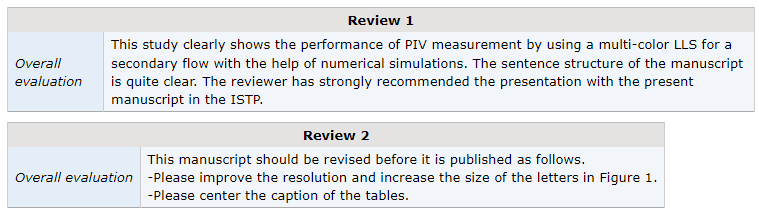
\includegraphics[width=90mm]{../images/reviews.png}
\end{figure}

\begin{itemize}
  \item 投稿内容の受理報告
  \item テーブルのキャプションの位置修正
  \item [※] 指摘に従って修正し,再投稿済み
\end{itemize}

\section{解析手順の再構成}
これまで検討を行ってきた解析の一連の流れとアルゴリズムについて,
性能向上と解析手順の明確化のため見直しを行っている.

\begin{enumerate}[(1)]
  \item [] \textgt{[ 全体の流れ ]}
  \item 校正ブロックの校正点特定と補正関数の取得
  \item 背景処理・粒子位置特定等の前処理
  \item 粒子追跡
  \item ベクトルの再配置・誤ベクトル除去等の後処理
\end{enumerate}

\subsection{(1) 校正プロックの校正点と補正関数の取得}
\begin{itemize}
  \item 24bitカラー画像から8bitグレイスケールへの変更を
        BT.601-5 に示される割合に従って変換
  \item 画素の周囲8要素を用いた中央値フィルタによってノイズを軽減
  \item 校正板の2値化画像生成時のしきい値を
        大津の2値化法に則って決定
  \item マスク画像を使用して校正点の中心点を取得
  \item 取得した校正点を用いて補正関数を計算
\end{itemize}

\newpage
\subsection{改善した内容}
\begin{itemize}
  \item メジアンフィルタによるごま塩ノイズの軽減
  \item しきい値の自動決定による二値化処理の統一
  \item 相互相間によるサブピクセル精度での校正点の特定
\end{itemize}

\begin{figure}[htbp]
  \begin{tabular}{cc}
    \begin{minipage}[t]{0.45\hsize}
      \centering
      
\includegraphics[keepaspectratio, width=40mm]{../images/original.bmp}
      \subcaption{Original}
    \end{minipage} &
    \begin{minipage}[t]{0.45\hsize}
      \centering
      \includegraphics[keepaspectratio, width=40mm]{../images/grayscale.bmp}
      \subcaption{Grayscale}
    \end{minipage} \\
    \begin{minipage}[t]{0.45\hsize}
      \centering
      \includegraphics[keepaspectratio, width=40mm]{../images/median.bmp}
      \subcaption{Median filter}
    \end{minipage}   &
    \begin{minipage}[t]{0.45\hsize}
      \centering
      \includegraphics[keepaspectratio, width=40mm]{../images/binary.bmp}
      \subcaption{Binarize}
    \end{minipage}
  \end{tabular}
  \caption{Calibration images}
  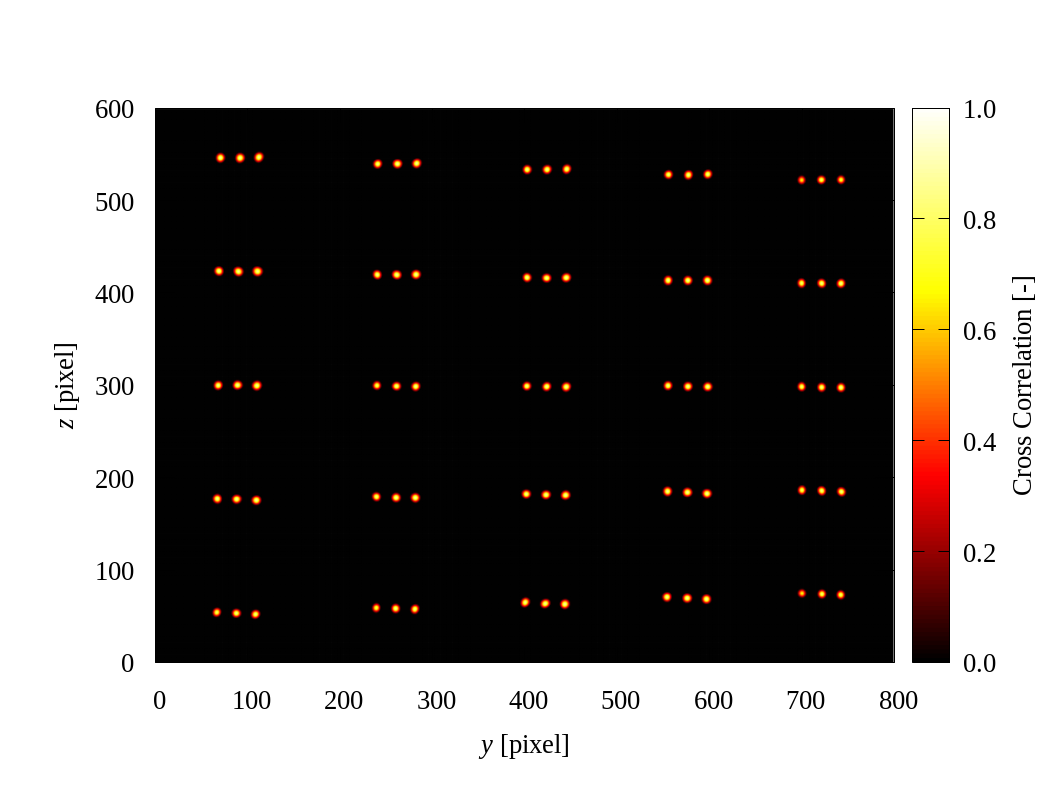
\includegraphics[keepaspectratio, width=82mm]{../images/cross_crr.png}
  \caption{Cross correlation of calibration image}
  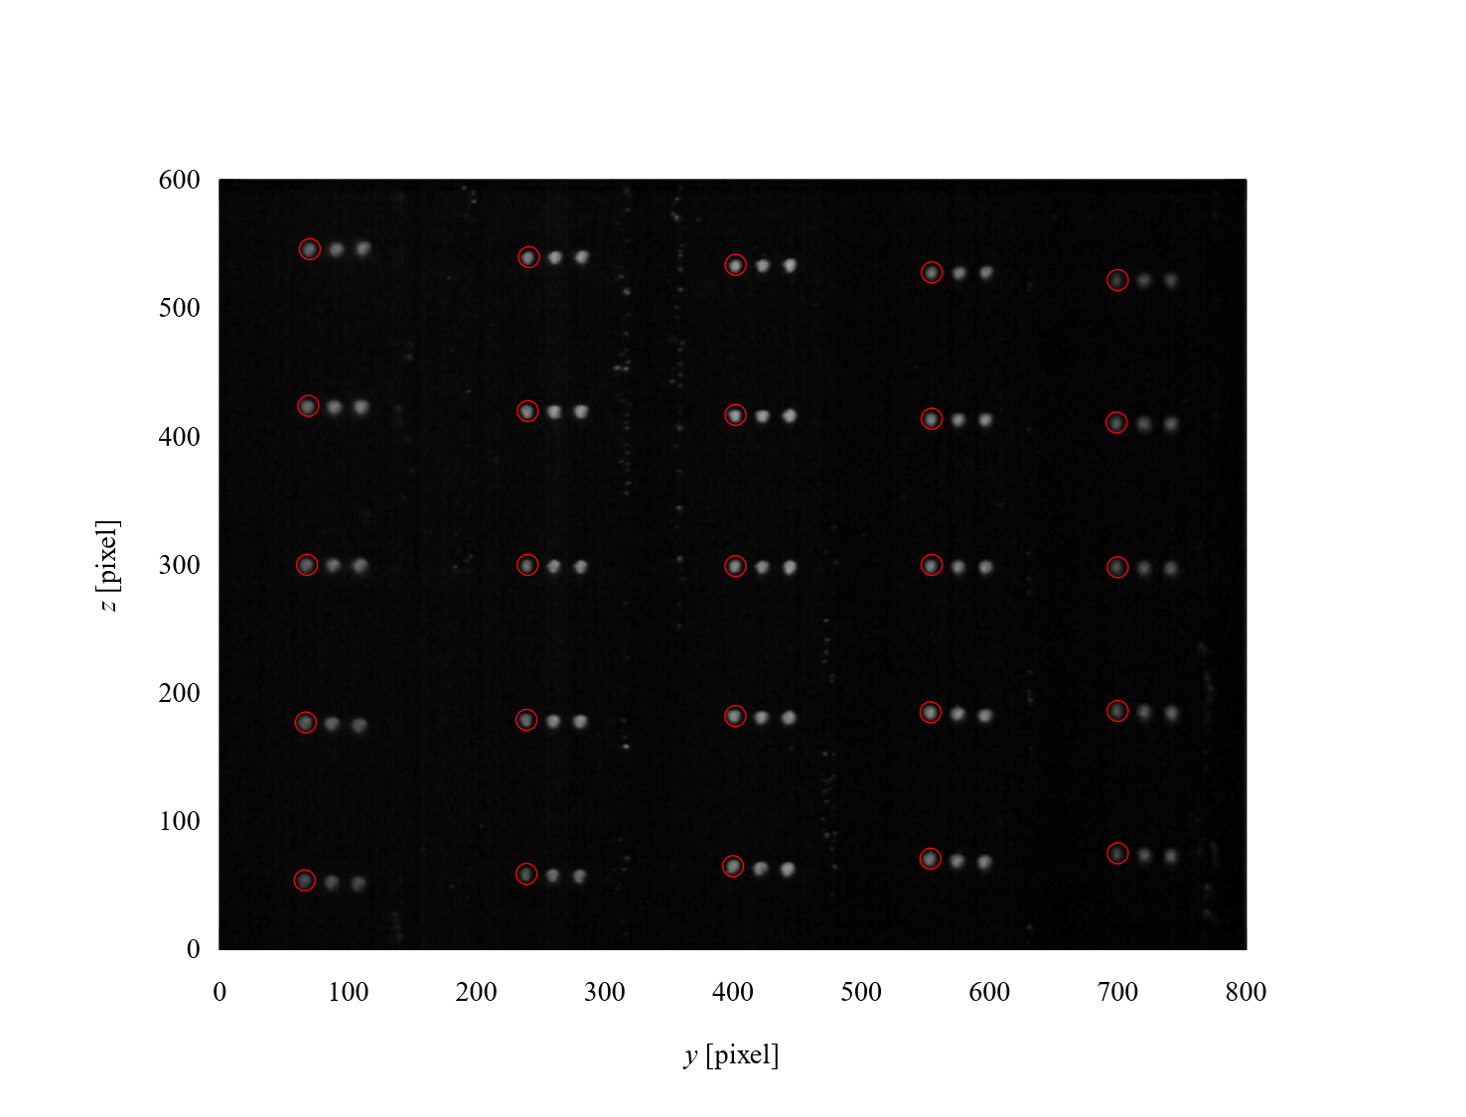
\includegraphics[keepaspectratio, width=82mm]{../images/calibration_0.png}
  \caption{Calibration points for left columns}
\end{figure}

\newpage
\subsection{(2) 背景処理と粒子位置の特定}
\begin{itemize}
  \item 撮影画像の平均値を用いた背景処理
  \item 混色の割合の計算し,カラーフィルタを作成
  \item カラーフィルタを用いた粒子像の識別 (B or G)
  \item 平均フィルタによる輝度分布の平滑化
  \item マスク画像を用いて粒子位置を特定
  \item 粒子位置を補正関数を用いて座標変換
\end{itemize}

\begin{figure}[htbp]
  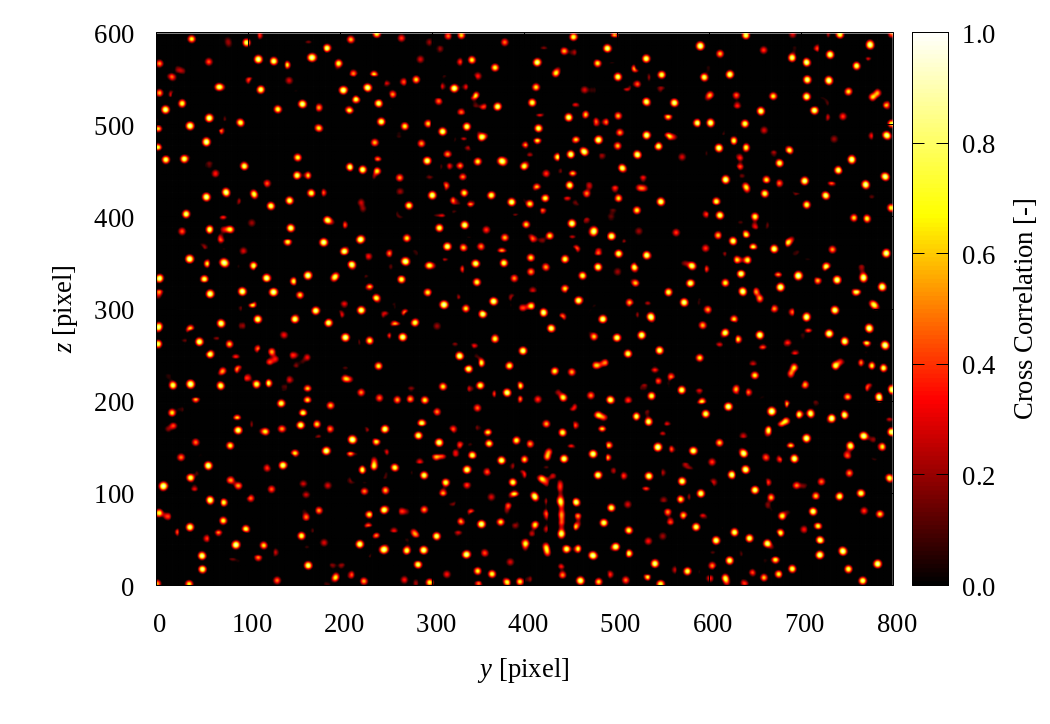
\includegraphics[keepaspectratio, width=82mm]{../images/cross_crr_particle.png}
  \caption{Cross correlation of particles image : Green}
  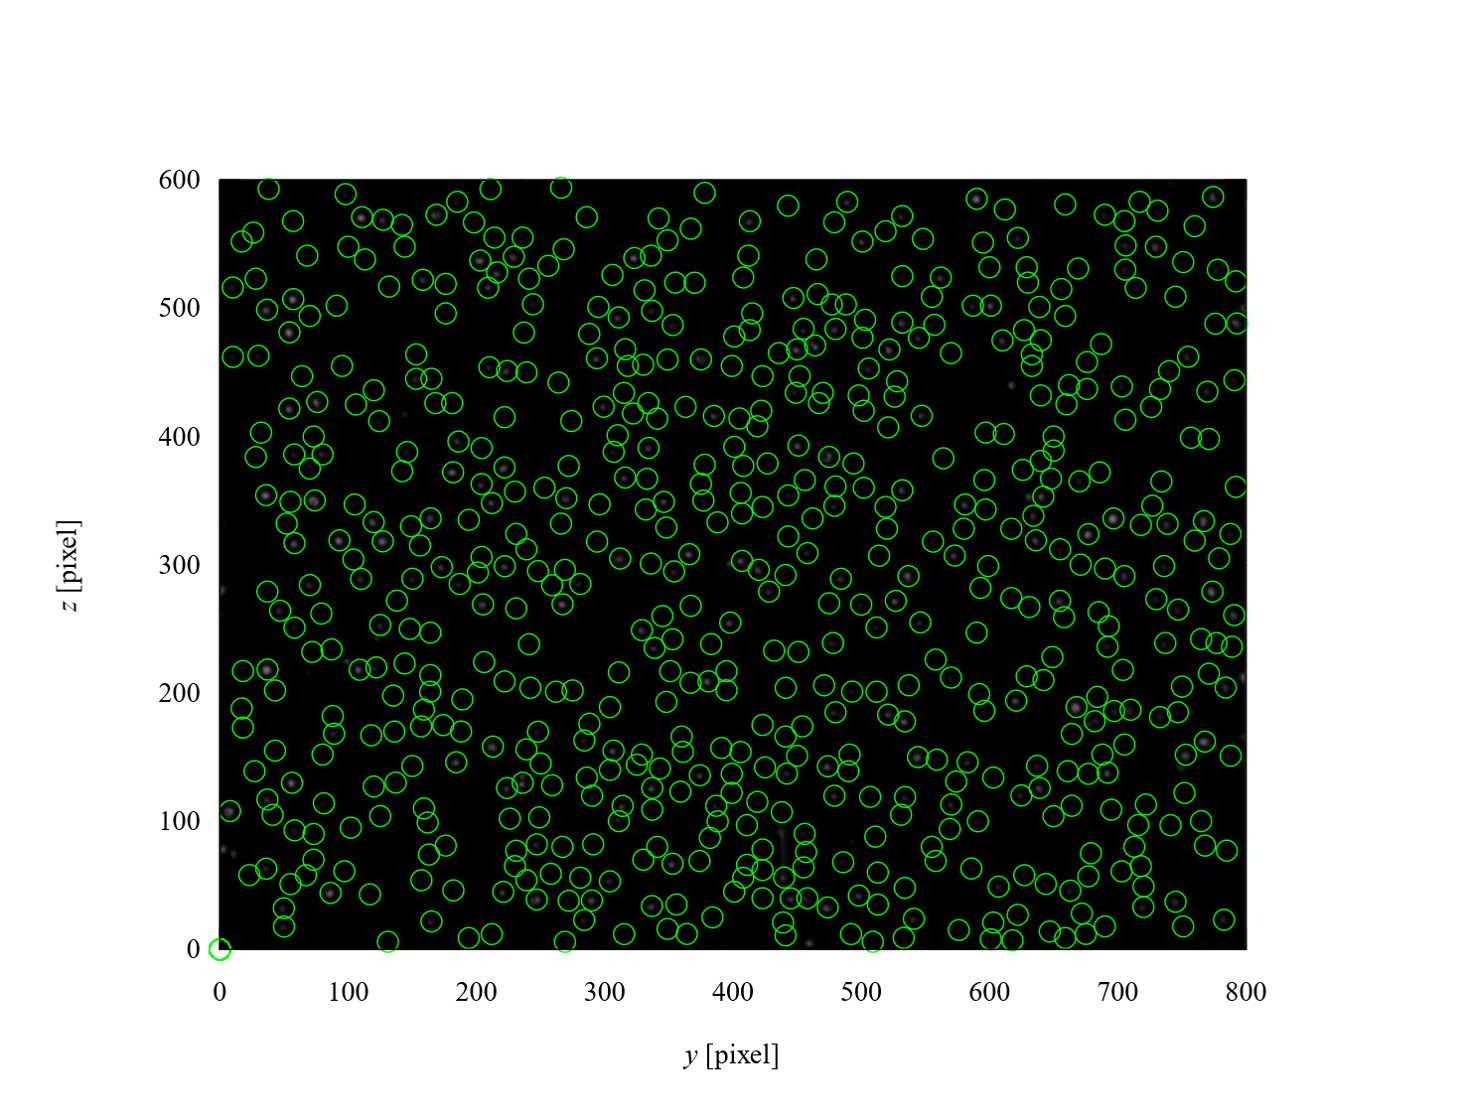
\includegraphics[keepaspectratio, width=82mm]{../images/particle_positions_green.png}
  \caption{Particles positions : Green}
\end{figure}

\subsection{改善した内容}
\begin{itemize}
  \item 相互相間によるサブピクセル精度の粒子位置特定
  \item 特定できる粒子数の大幅な増加
\end{itemize}

\begin{table}[hbtp]
  \centering
  \caption{Particle detection for green image}
  \begin{tabular}{l c}
    \hline
    Method of particle detection & Number of particles \\ \hline \hline
    Binarization image           & 100                 \\ \hline
    Cross correlation plane      & 200                 \\ \hline
  \end{tabular}
\end{table}



\section{9月の予定}
\begin{itemize}
  \item ISTP-33 (9/24 - 27)
  \item 解析手順の再構成 (続き)
\end{itemize}

\end{document}